
\section{Background}
\label{sec-mot}

This section gives more background on dmck and related terms,
followed with a detailed overview of the state of the art.  

%Then, we present cases of deep bugs and motivate the need for dmck
%advancements.


\subsection{DMCK Framework and Terms}
\label{mot-bgterms}


As mentioned before, we define {\em dmck} as  software model checker
that checks distributed systems directly at the implementation level.
Figure~\ref{fig-dmck} illustrates a dmck integration to a target
distributed system, a simple representation of existing dmck
frameworks~\cite{Guo+11-Demeter, Killian+07-LifeDeathMaceMC,
  Simsa+10-Dbug, Yang+09-Modist}.  The dmck inserts an interposition
layer in each node of the target system with the purpose of
controlling all important events (\eg, network messages, timeouts) and
preventing the target system to process the events until the dmck
enables them.  A main dmck mechanism is the permutation of events; the
goal is to push the target system into all possible ordering scenarios.
For example, the dmck can enforce \ts{abcd} ordering in one execution,
\ts{bcad} in another, and so on.



% List all the terms
We now provide an overview of basic dmck terms we use in this paper
and Figure~\ref{fig-dmck}.
%
Each node of the target system has a {\em local state} (\ls),
containing many variables.  An {\em abstract local state} (\als) is a
subset of the local state; dmck decides which \als\ is important to
check.
%
The collection of all (and abstract) local states is the {\em global
  state} (\gs) and the {\em abstract global state} (\ags)
respectively.  
%
The {\em network state} describes all the {\em outstanding messages}
currently intercepted by dmck (\eg, \ts{abd}).
%
To model check a specific protocol, dmck starts a {\em workload
  driver} (which restarts the whole system, runs specific workloads,
\etc).  Then, dmck generates many (typically hundreds/thousands)
executions; an {\em execution} (or a {\em path}) is a specific
ordering of events that dmck enables (\eg, \ts{abcd}, \ts{dbca}) from
an initial state to a termination point.
%
A {\em sub-path} is a subset of a path/execution.
%
An {\em event} is an action by the target system that is intercepted
by dmck (\eg, a network message) or an action that dmck can inject
(\eg, a crash/reboot).
%
Dmck enables one event at a time (\eg, \ts{enable(c)}).
%
To permute events, dmck runs {\em exploration methods} such as
brute-force (\eg, depth first search) or random.  
%
%
As events are permuted, the target system enters hard-to-reach
states.  Dmck continuously runs state {\em checks} (\eg, safety 
checks) to verify the system's correctness.
%
To reduce the state-space explosion problem, dmck can employ {\em
  reduction policies} (\eg, DPOR or symmetry).  A policy is {\em
  systematic} if it does not use randomness or bug-specific knowledge.
%
In this chapter, we focus on advancing systematic reduction policies.




\subsection{State-of-the-Art DMCKs}
\label{mot-samc-state}



% dpor /  modist
\modist~\cite{Yang+09-Modist} is arguably one of the most powerful dmcks that
comes with systematic reduction policies.  \modist\ has been integrated to real
systems due to its exploration scalability.  At the heart of \modist\ is {\em
dynamic partial order reduction (DPOR)}~\cite{Flanagan+05-Dpor} which exploits
the {\em independence} of events to reduce the state explosion.  Independent
events mean that it does not matter in what order the system execute the
events, as their different orderings are considered equivalent.

To illustrate how \modist\ adopts DPOR, let's use the example in
Figure~\ref{fig-samc-dmck}, which shows four concurrent outstanding messages
\ts{abcd} (\ma\ and \mb\ for \none, \mc\ and \md\ for \ntwo).  A brute-force
approach will try all possible combinations (\ts{abcd}, \ts{abdc}, \ts{acbd},
\ts{acdb}, \ts{cabd}, and so on), for a total of 4!  executions.
% dpor
Fortunately, the notion of event independence can be mapped to distributed
system properties.  For example, \modist\ specifies this reduction policy: a
message to be processed by a given node is independent of other concurrent
messages destined to other nodes (based on vector clocks).  Applying this
policy to the example in Figure~\ref{fig-samc-dmck} implies that \ma\ and \mb\ are
dependent\footnote[1]{In model checking, ``dependent'' events mean that they
must be re-ordered.  ``Dependent'' does not mean ``causally dependent''.}  but
they are independent of \mc\ and \md\ (and vice versa).  Since only dependent
events need to be reordered, this reduction policy leads to only 4 executions
(\ma\mb-\mc\md, \ma\mb-\md\mc, \mb\ma-\mc\md, \mb\ma-\md\mc), giving a 6x
speed-up (4!/4).


\begin{figure}

\centerline{
%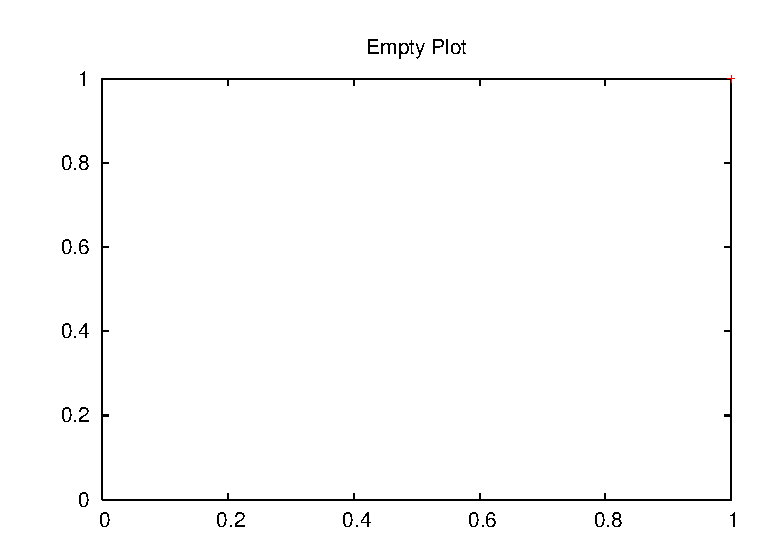
\includegraphics[height=1in]{F/empty.eps}
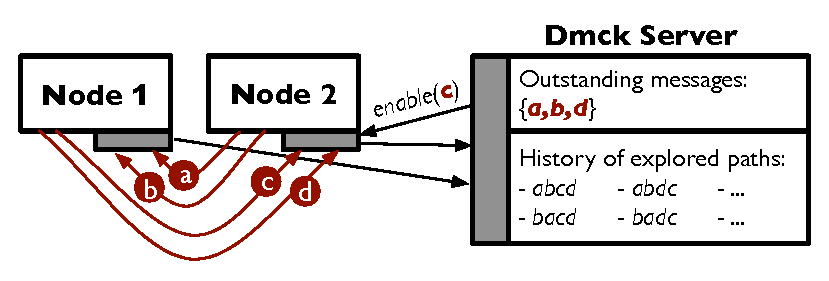
\includegraphics[height=1.7in]{F/dmck/dmck-simple.eps}
}
\vminfive
\mycaption[How dmck works]{fig-samc-dmck}{How dmck works}{A scenario when a dmck is
working and there are four concurrent messages sent to two nodes (Node 1 and
Node 2).
}
%\vminten
\end{figure}

 % -- pics

Although \modist's speed-up is significant, we find that one
scalability limitation of its DPOR application is within its {\em
  black-box} approach; it only exploits general properties of
distributed systems to define message independence.  It does not
exploit any semantic information from the target system to define more
independent events.  We will discuss this issue later
(\sec\ref{sec-samc-semantic}).



%




\begin{figure*}[t]

\centerline{
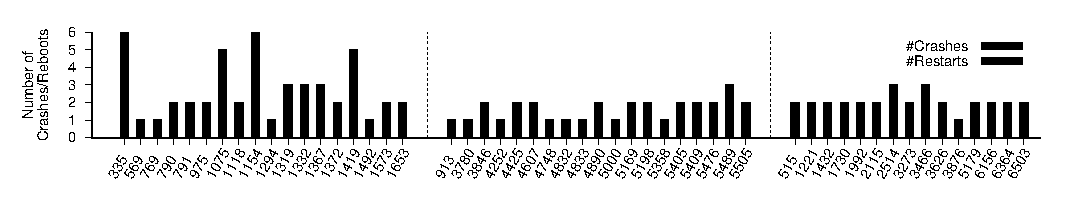
\includegraphics[width=6.5in]{F/deepbugs/eps/all.eps}
%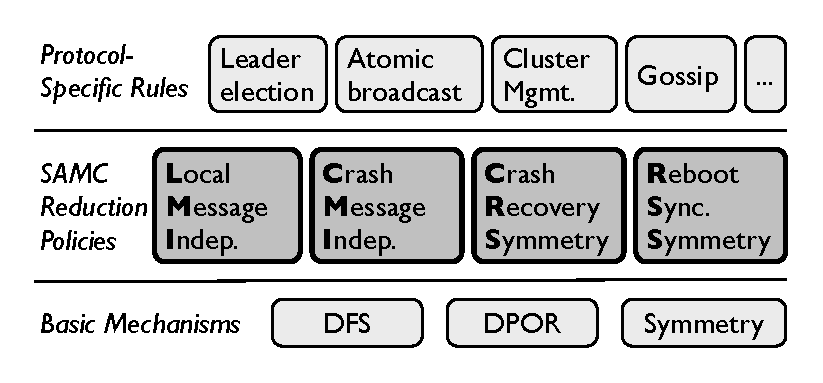
\includegraphics[height=1.2in]{F/samc/samc.eps}
}
\scriptsize{
~~~~~~~~~~~~~~~~~~~~~~~~~~~~~~~~~~~~~~\textsf{ZooKeeper Bugs}
~~~~~~~~~~~~~~~~~~~~~~~~~~~~~~~~~~~~\textsf{Hadoop MapReduce Bugs}
~~~~~~~~~~~~~~~~~~~~~~~~~~~~~~~\textsf{Cassandra Bugs}}
\vminfive
\mycaption[Deep Bugs]{fig-deepbugs}{Deep Bugs}{
%
The figure lists deep bugs from our bug study and depicts how many
crashes and reboots must happen to reproduce the bugs. Failure events
must happen in a specific order in a long sequence of events.  These
bugs came from many protocols including ZooKeeper leader election and
atomic broadcast, Hadoop MapReduce speculative execution, job/task
trackers, and resource/application managers, and Cassandra gossiper,
anti-entropy, mutation, and hinted handoff.  These bugs led to failed
jobs, node unavailability, data loss, inconsistency, and corruption.
They were labeled as ``major'', ``critical'', or ``blocker''.  12 of
these bugs happened within the last one year.  The median response
time (\ie, time to fix) is two weeks. There are few bugs that involve
4+ reboots and 4+ crashes that we do not show here.
%
} 
%\vminten

\end{figure*}

 % -- pics

% ------------------------------------------------------

% deemter
Dynamic interface reduction (DIR)~\cite{Guo+11-Demeter} is the next
advancement to \modist.  This work suggests that a complete dmck must
re-order not only messages (global events) but also thread
interleavings (local events).  The reduction intuition behind DIR is
that different thread interleavings often lead to the same global
events (\eg, a node sends the same messages regardless of how threads are
interleaved in that node).  DIR records local exploration and replays
future incoming messages without the need for global exploration.  
In our work, SAMC focuses only on global exploration (message and failure
re-orderings).  We believe DIR is orthogonal to SAMC, similar to the
way DIR is orthogonal to \modist.


% besides (quick take)
\modist\ and DIR are examples of dmcks that employ advanced systematic
reduction policies.  LMC~\cite{Guerraoui+11-McNoNetwork} is similar to
DIR; it also decouples local and global exploration.
dBug~\cite{Simsa+10-Dbug} applies DPOR similarly to \modist.  There are
other dmcks such as \macemc~\cite{Killian+07-LifeDeathMaceMC} and
CrystalBall~\cite{Yabandeh+09-CrystalBall} that use basic exploration
methods such as depth first (DFS), weight-based,
and random searches.

% symmetry
Other than the aforementioned methods, {\em symmetry} is another
foundational reduction policy~\cite{Emerson+97-PorAndSym,
  Prasad+00-SymBasedMc}.  Symmetry-based methods exploit the
architectural symmetry present in the target system.  For example, in
a ring of nodes, one can rotate the ring without affecting
the behavior of the system.  Symmetry is powerful, but 
we find no existing dmcks that adopt symmetry.

% multiple failures
Besides dmcks, there exists sophisticated testing frameworks for
distributed systems (\eg, \fate~\cite{Gunawi+11-FateDestini},
\prefail~\cite{Joshi+11-PreFail},
\setsudo~\cite{Joshi+13-SetsudoTesting}, OpenStack
fault-injector~\cite{Ju+13-FaultResOpenStack}). This set of work
emphasizes the importance of multiple failures, but their major
limitation is that they are not a dmck.  That is, they cannot
systematically control and permute non-deterministic choices such as
message and failure reorderings.


\subsection{Does State of the-Art Help?}
\label{mot-summ}

We now combine our observations in the previous section and our insight from
\taxdc\ (Chapter \ref{chp-taxdc}), and describe why state-of-the-art dmcks do
not address present reliability challenges of cloud systems.

% policies and bugs, random
First, {\em existing systematic reduction policies often cannot find bugs
quickly}.  Experiences from previous dmck developments suggest that significant
savings from sound reduction policies do not always imply high bug-finding
effectiveness~\cite{Guo+11-Demeter, Yang+09-Modist}.  To cover deep states and
find bugs, many dmcks revert to non-systematic methods such as randomness or
manual checkpoints.  For example, \modist\ combines DPOR with random walk to
``jump'' faster to a different area of the state space (\sec4.5
of~\cite{Yang+09-Modist}).  DIR developers find new bugs by manually setting
``interesting'' checkpoints so that future state explorations happen from the
checkpoints (\sec5.3 of~\cite{Guo+11-Demeter}).  In our work, although we use
different target systems, we are able to reproduce the same experiences above
(\sec\ref{eval-oldbugs}).



% multiple failures
Second, {\em existing dmcks do not scale with the inclusion of failure events}.
Given the first problem above, exercising multiple failures will just exacerbate
the state-space explosion problem.  Some frameworks that can explore multiple
failures such as \macemc~\cite{Killian+07-LifeDeathMaceMC} only do so in a
random way; however, in our experience (\sec\ref{eval-oldbugs}), randomness many
times cannot find deep bugs quickly.  \modist\ also enabled only one failure.
In reality, multiple failures is a big reliability threat, and thus must be
exercised.


We conclude that finding systematic (no random/checkpoint) policies that can
find deep bugs is still an open dmck research problem.  We believe without
semantic knowledge of the target system, dmck hits a scalability wall (as also
hinted by DIR authors; \sec8 of~\cite{Guo+11-Demeter}).  In addition, as crashes
and reboots need to be exercised, we believe recovery semantics must be
incorporated into reduction policies.  All of these observations led us to SAMC,
which we describe next.



